\section{Введение}
Лабораторная работа по курсу "Алгоритмы и анализ сложности". Алгоритм Грэхема: с использованием быстрой сортировки и с использованием сортировки, основанной на АВЛ-дереве.

\subsection{Постановка задачи}

\noindent \textbf{Постановка задачи построения выпуклой оболочки}\\
\indent Для точек $a_1, ..., a_n$, где $n\geq1$, $a_i=(a_{i,1},a_{i,2})\in R^2$ при $i=1,...,n$, указать вершины $b_1,...,b_m$ выпуклой оболочки $Conv(a_1,...,a_n)$ в порядке их встречи при движении по ее границе. В общем случае $Conv(a_1,...,a_n)$ является многоугольником, а в вырожденных случаях может получиться отрезок или точка. В случае отрезка выходом алгоритма, решающего поставленную задачу, должны быть две точки, являющиеся его концами точки, а в случае точки -- сама эта точка.

\noindent \textbf{Цель лабораторной работы}\\
\indent Сравнение и анализ двух алгоритмов, решающих задачу: алгоритм Грэхема с использованием быстрой сортировки, алгоритм Грэхема с использованием сортировки, основанной на АВЛ-дереве.

\noindent \textbf{План лабораторной работы}:
\begin{enumerate}
	\item{($Program1$) Первая программа: чтение из файла входных данных, на выходе - файл с результатами работы алгоритма и временем работы.}
	\item{($Program2$) Вторая программа: проведение экспериментов над реализованными алгоритмами:
		\begin{itemize}
			\item[--]{Генератор тестов для проведения экспериментов, в котором можно выбрать:
				\begin{itemize}
					\item[+]{Кол-во точек $n$ в исходном массиве $a$.}
					\item[+]{Натуральные числа $q$ и $w$.}
					\item[+]{Режимы: ($A$) псевдослучайные точки в прямоугольнике со сторонами $q$ и $w$, ($B$) псевдослучайные точки на границе (на сторонах) этого прямоугольника.}
			\end{itemize}}
			\item[--]{Провести следующие эксперименты:
				\begin{itemize}
					\item[+]{($E1$) $q = 10^6, w = 10^6$, $n = 1, ..., 10^6+1$ с шагом $10^4$ в режимах ($A$) и ($B$). Построить графики $T_A(n)$ и $T_B(n)$.}
					\item[+]{($E2$) $q = w = 0, ..., 10^6$ с шагом $10^4$, $n = 10^6$ в режимах ($A$) и ($B$). Построить графики $T_A(q)$ и $T_B(q)$.}
			\end{itemize}}
		\end{itemize}
	}
	\item{Сформулировать и обосновать вывод о том, в каких случаях целесообразно применять какой из алгоритмов.}
\end{enumerate}

\subsection{Структура проекта}
\noindent \textbf{Program1}: Реализация первой программы ($Program1$):\\
Файлы: /Program1/main.cpp\\
\noindent \textbf{Program2}: Реализация второй программы ($Program2$):\\
Файлы: /Program2/main.cpp\\
\noindent \textbf{GrahamScan}: Реализация алгоритма Грэхема:\\
Файлы: /GrahamScan/GrahamScan.h, /GrahamScan/GrahamScan.cpp\\
\noindent \textbf{QuickSort}: Реализация быстрой сортировки:\\
Файлы: /QuickSort/QuickSort.h, /QuickSort/QuickSort.cpp\\
\noindent \textbf{AVLTree}: Реализация АВЛ-дерева:\\
Файлы: /AVLTree/AVLTree.h, /AVLTree/AVLTree.cpp\\
\noindent \textbf{Utils}: Общие функции и классы, необходимые для реализации алгоритмов:\\
Файлы: /Utils/Utils.h, /Utils/Utils.cpp\\
\noindent \textbf{Utils\_IO}: Функции для ввода и вывода:\\
Файлы: /Utils/Utils\_IO.h, /Utils/Utils\_IO.cpp\\
\noindent \textbf{Utils\_TestGen}: Функции для генерации тестов:\\
Файлы: /Utils/Utils\_TestGen.h, /Utils/Utils\_TestGen.cpp\\

\begin{figure}[h]
	\centering
	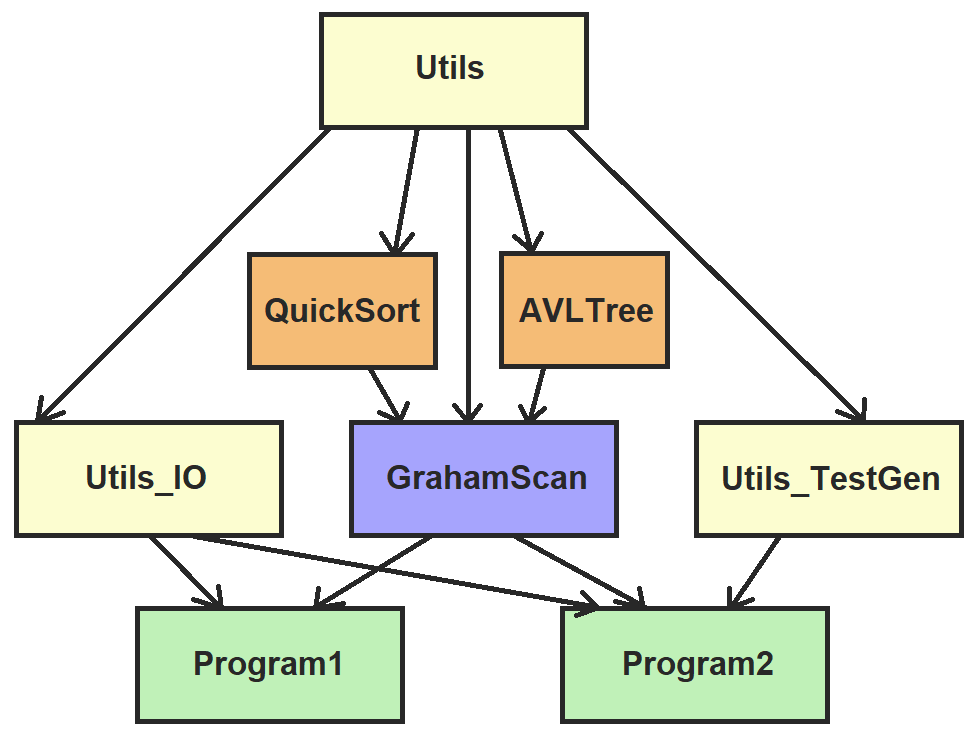
\includegraphics[width=0.7\textwidth]{Images/project_structure.png}
	\caption{Граф зависимостей}
	\label{fig:project_structure}
\end{figure}

\newpage
